\section{Some examples}

First we will compute some examples using knowledge previously
discussed about the \grob fan.

\begin{example}
  Let us consider the polynomial ring $\mathbb{Q}[x, y, z]$ and
  the ideal $\{yz + x, xy + z, x^2 -z^2\}$. We can start the computation
  of the marked \grob basis by taking the graded lexicographical order for
  all the possible variable orderings. We obtain:

  \begin{itemize}
  \item Graded reverse lexicographic order $x > y > z$: $\{(yz)+x, (xy)+z, (x^2)-z^2\}$
  \item Graded reverse lexicographic order $x > z > y$: $\{(yz)+x, (xy)+z, (x^2)-z^2\}$
  \item Graded reverse lexicographic order $y > x > z$: $\{(yz)+x, (x^2)-z^2, (xy)+z\}$
  \item Graded reverse lexicographic order $y > z > x$: $\{(xy)+z, (z^2)-x^2, (yz)+x\}$
  \item Graded reverse lexicographic order $z > x > y$: $\{(xy)+z, (yz)+x, (z^2)-x^2\}$
  \item Graded reverse lexicographic order $z > y > x$: $\{(xy)+z, (yz)+x, (z^2)-x^2\}$
  \end{itemize}

  Essencially there are only two different marked \grob bases. Are these all the marked \grob bases?
  We can check this in two ways, using a geometric approach or using the algorithm above. The
  geometric approach it is indeed inefficient since it requires to check if the set of cones
  cover the positive orthant of $\real^n$. If the entire positive orthant of $\real^n$ is covered
  then we stop, otherwise we choose a vector in the complement area of the cones space generated so far.

  We will use the geometric approach. For the latter, we notice the current set of cones produced
  by the marked \grob bases is shown in Figure 2 (Left):

  \begin{figure}[h]
    \centering
    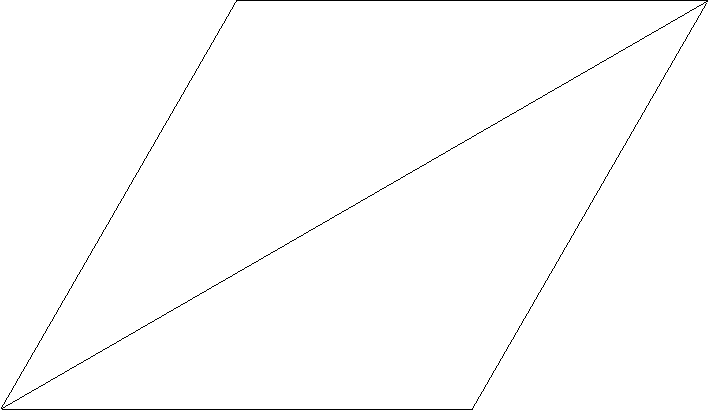
\includegraphics[width=5cm]{workingExample1}
    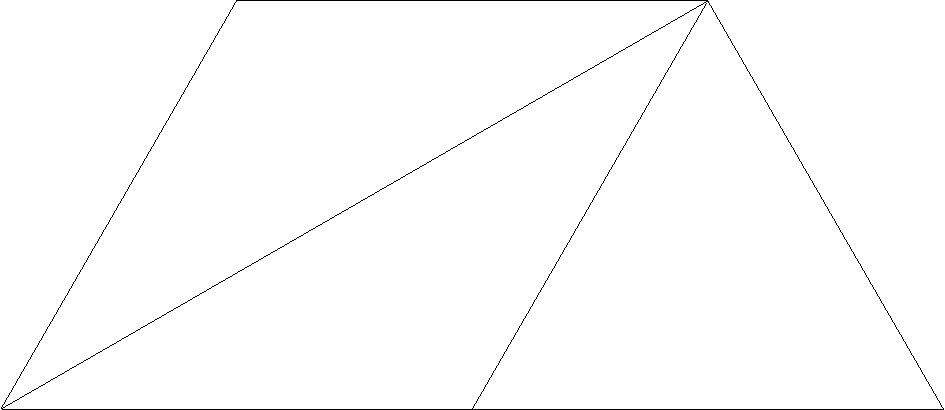
\includegraphics[width=5cm]{workingExample2}
    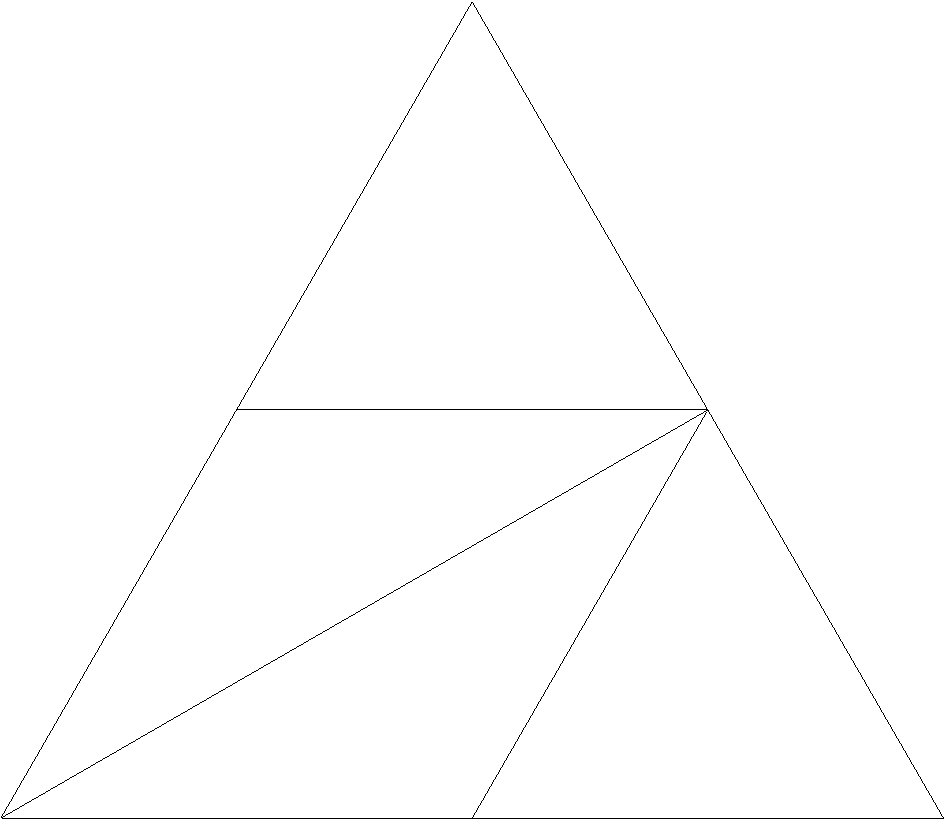
\includegraphics[width=5cm]{ideal2}
    \caption{Cones of the progressive computation for the \grob fan of the ideal
      $\{yz + x, xy + z, x^2 -z^2\}$}
  \end{figure}

  Using the \emph{gfanInterface} \cite{gfan} from Macaulay2 \cite{M2} we observe the render produced
  intersect the cone with the hyperplane $x + y + z = 1$ in order to produce a 2D plot. From this
  fact we know the set of cones cover the positive orthant of $\real^3$ when the render forms a triangle.
  Hence, we can choose a vector ($w = (1, 0, 0)$) from the bottom right side. From the latter
  we obtain the marked \grob basis (the correspondent set of cones is in Figure 2 (Center)) $\{(y^2*z) -z, (x) + y*z\}$.
  Now we try to extend the cones with the vector $w = (0, 0, 1)$ and we obtain the marked \grob
  basis $\{(x*y^2) -x, (z) + x*y\}$. The final set of cones is shown in Figure 2 (Right). Since
  the latter intersects with the triangle mention before we are sure we have computed all the
  marked \grob bases for the ideal $\{yz + x, xy + z, x^2 -z^2\}$.
\end{example}

\begin{example}
  Let us consider the polynomial ring $\mathbb{Q}[x, y, z]$ and
  the ideal $\{x*y - x, x^2 + x*z, y^2*z + x\}$. For this example we will
  use our implementation of the Mora and Robbiano algorithm.

  \begin{itemize}
  \item First we compute all the possible monomial orders. Enumerating all the possibilities
    these are the potential candidates:
  \end{itemize}
\end{example}


%%% Local Variables: 
%%% mode: latex
%%% TeX-master: "main"
%%% End: 